\documentclass[11pt]{beamer}
\usetheme{Pittsburgh}

\setbeamertemplate{navigation symbols}{%
    \insertslidenavigationsymbol 	\insertframenavigationsymbol 	\insertsubsectionnavigationsymbol 	\insertsectionnavigationsymbol 	\insertdocnavigationsymbol 	\insertbackfindforwardnavigationsymbol 	\hspace{1em}%
    \usebeamerfont{footline} 	\insertframenumber/\inserttotalframenumber%
}

%% Packages:

\usepackage[utf8]{inputenc}

\usepackage{amsmath}
\usepackage{amsfonts}
\usepackage{amssymb}

\usepackage{graphicx}

\usepackage{listings}
\lstset{escapeinside={<@}{@>}}

\usepackage{appendixnumberbeamer}

%% Definitions:

\definecolor{codegreen}{rgb}{0,0.6,0}
\definecolor{codegray}{rgb}{0.5,0.5,0.5}
\definecolor{codepurple}{rgb}{0.58,0,0.82}
\definecolor{backcolour}{rgb}{0.95,0.95,0.92}

\lstdefinestyle{mystyle}{
    backgroundcolor=\color{backcolour},   
    commentstyle=\color{codegreen},
    keywordstyle=\color{magenta},
    numberstyle=\tiny\color{codegray},
    stringstyle=\color{codepurple},
    basicstyle=\ttfamily\scriptsize,
    breakatwhitespace=false,         
    breaklines=true,                 
    captionpos=b,                    
    keepspaces=true,                 
    numbers=left,                    
    numbersep=5pt,                  
    showspaces=false,                
    showstringspaces=false,
    showtabs=false,                  
    tabsize=2
}
\lstset{style=mystyle}
\lstset{language=c++}

\newcommand{\tlapack}{{$\langle$T$\rangle$LAPACK }}
\newcommand{\cpp}{{C\texttt{++}}}
\newcommand{\BLASPP}{{BLAS\texttt{++}}}
\newcommand{\LAPACKPP}{{LAPACK\texttt{++}}}

%% Comments:

\newcommand{\wes}[1]{{\color{red} #1}}


%% Title:

\author{Weslley da Silva Pereira, University of Colorado Denver}
\title{Exception handling for the BLAS and LAPACK}
%\setbeamercovered{transparent} 
%\setbeamertemplate{navigation symbols}{} 
% \titlegraphic{\flushright 
\includegraphics[height=.15\linewidth]{img/NSF}} 
% \institute{University of Colorado Denver} 
\date{BLIS Retreat 2022\\\vspace{10pt} September 22, UT Austin}
%\subject{}

\begin{document}

\begin{frame}
\titlepage
\end{frame}

\begin{frame}{Coauthors~\footnote{Proposed Exception Handling
	for the BLAS and LAPACK:\\ \url{https://www.arxiv.org/abs/2207.09281}}}

	\begin{itemize}
		\item Jim Demmel, UC Berkeley,
		\item Jack Dongarra, U Tennessee, Knoxville,
		\item Mark Gates, U Tennessee, Knoxville,
		\item Greg Henry, Intel Corp.,
		\item Julien Langou, U Colorado, Denver,
		\item Xiaoye Li, LBNL,
		\item Piotr Luszczek, U Tennessee, Knoxville,
		\item Weslley Pereira, U Colorado, Denver,
		\item Jason Riedy, Lucata Corp.,
		\item Cindy Rubio-Gonzalez, UC Davis.
	\end{itemize}
	
\end{frame}

\begin{frame}{Examples of bad exception handling}

	\begin{itemize}
		\item Ariane 501, 1996. ``[An] exception was caused during execution of a data conversion from 64-bit floating point to 16-bit signed integer value.''~\footnote{\url{https://www-users.cse.umn.edu/~arnold/disasters/ariane.html}}
		\item Roborace, 2020. ``the system somehow managed to produce a NaN (not a number) value and all verification logic was designed to work only with numbers.''~\footnote{\url{https://www.reddit.com/r/formula1/comments/jk9jrg/comment/gai295l}}
	\end{itemize}

	\vspace{10pt}
	\begin{center}
		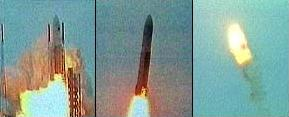
\includegraphics[width=.53\linewidth]{img/ariane}
		\hfill
		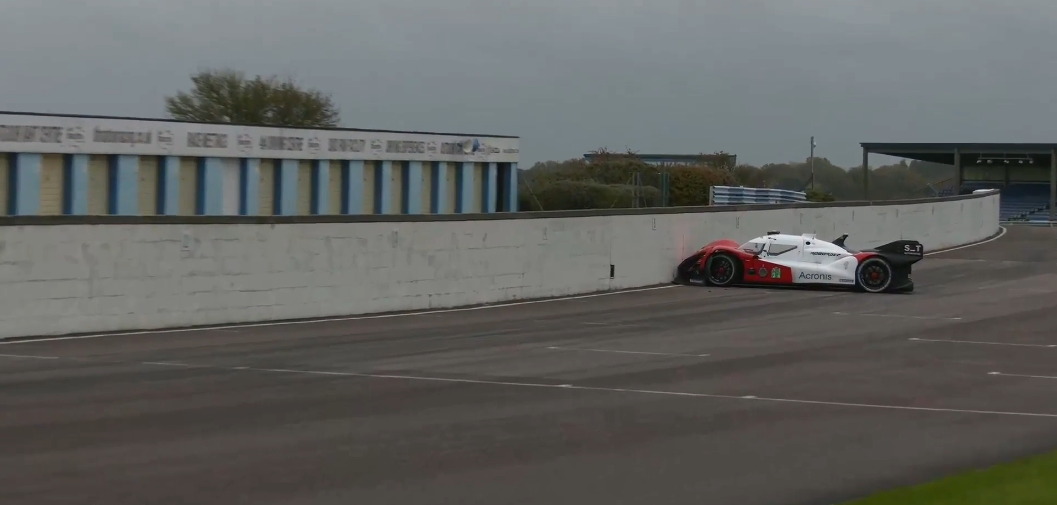
\includegraphics[width=.45\linewidth]{img/roborace}
	\end{center}
\end{frame}

\begin{frame}{Agenda}

	\tableofcontents

	\begin{center}
		One of the goals of this talk:\\
		\textbf{Seek feedback}
	\end{center}

\end{frame}

\section{Inconsistencies in the Reference BLAS and LAPACK libraries (Some also in BLIS)}

\begin{frame}{Inconsistencies in the Reference BLAS}

	IxAMAX: Return the index of the largest entry.
	\begin{itemize}
		\item Inconsistency \#1:\\
		~ \texttt{isamax([ 0, NaN, 2 ]) = 3},\\
		~ \texttt{isamax([ NaN, 0, 2 ]) = 1},
		\item Inconsistency \#2:\\
		~ \texttt{icamax([ OV+i*OV, Inf+i*0 ]) = 1},\\
		~ \texttt{icamax([ .6*OV+i*.6*OV, .7*OV+i*.7*OV ]) = 1},\\
		where \texttt{OV} is the overflow threshold.
		\item Proposed consistent fix: 
	\end{itemize}

	\begin{center}
		\textbf{Return index to the first NaN,\\ else to the first Inf,\\ else to the first largest finite entry.}
	\end{center}
	
	% ~\\
	% \begin{itemize}
	% 	\item \textbf{Challenge:} This (inconsistent) behavior is a standard!
	% \end{itemize}

	\only<2>{\footnotesize \flushright \color{red} BLIS 0.9.0 has inconsistency \#2 only.}

\end{frame}

\begin{frame}{Inconsistencies in the Reference BLAS}

	xGER: $A := A + \alpha x y^T$.
	\begin{itemize}
		\item Current Reference BLAS:\\
		~ If $\alpha = 0$, return $A$.\\
		~ If $y_j = 0$ then $A_{ij} := A_{ij}$. ( What if $x_i = Inf$ or $NaN$? )\\
		~ There is no check for $x_i = 0$.
	\end{itemize}

	~\\
	xTRSV: Solve $Tx = b$ for $x$.
	\begin{itemize}
		\item Current Reference BLAS:\\
		~ Skip trailing 0s in $b$.\\
		~ If $x_j = 0$ then skip update $x_i := x_i - T_{ij}x_j$.\\
		~ No checks for 0s when solving $T^Tx = b$.
	\end{itemize}

	~\\
	Proposed consistent fix:
	\begin{center}
		\textbf{Keep check for $\alpha = 0$ but not for $x_i = 0$, $y_i = 0$ or $b_i = 0$.}
	\end{center}

	% ~\\
	% \begin{itemize}
	% 	\item \textbf{Challenge:} This (inconsistent) behavior is a standard!
	% \end{itemize}

\end{frame}

\begin{frame}{Inconsistencies in LAPACK}

	xGETF2 + xGETRS: Solve $Ax=b$ for $x$.

	~\\
	\begin{itemize}
		\item Example:
		$A = \begin{bmatrix}
			1 & 0\\
			NaN & 2
		\end{bmatrix}$ and 
		$b = \begin{bmatrix}
			0\\
			1
		\end{bmatrix}$.
		\item Combination of inconsistencies in the Reference BLAS:
		\begin{itemize}[<+->]
			\item \texttt{IxAMAX} chooses $A_{11} = 1$, not $A_{21} = NaN$, as pivot.
			\only<1>{$$A = \begin{bmatrix}
				\smash{\color{red}\fbox{\color{black}\rule[-15pt]{0pt}{1pt}$\;\, 1 \;\,$}} & 0\\
				NaN & 2
			\end{bmatrix}$$}
			\item \texttt{xGER} finds $0$ in $A_{12}$ and does not use the NaN. \only<2>{{\tiny \color{red} (Also on BLIS 0.9.0)}}
			\only<2>{$$A_{22} := A_{22} \textcolor{red}{- NaN \cdot 0}$$}
			\item LU factorization:
			$L = \begin{bmatrix}
				1 & 0\\
				NaN & 1
			\end{bmatrix}, \quad U = \begin{bmatrix}
				1 & 0\\
				0 & 2
			\end{bmatrix}$
			\item The first call for \texttt{xTRSV} solves $Ly=b$ and finds $y = \begin{bmatrix}
				0\\ 1
			\end{bmatrix}$.
			\only<4>{In the second iteration, $y_2 := 1 {\color{red}- NaN \cdot y_1}$ and $y_1=0$.}
			\item The final solution is $x = \begin{bmatrix}
				0\\
				0.5
			\end{bmatrix}$
		\end{itemize}
		\only<5>{\item \textbf{NaN does not propagate!}}
	\end{itemize}

	\only<5>{\flushright\footnotesize \color{red} BLIS 0.9.0 propagates NaNs in this example.}

\end{frame}

% \section{Inconsistencies between languages and compilers}

\begin{frame}[fragile]{Examples of unavoidable inconsistencies}

	Summation order: \texttt{sum([OV,OV,-OV,-OV])} can be\\
	~\texttt{NaN, Inf, -Inf} or \texttt{0}, ~ where \texttt{OV} is the overflow threshold.

	
	~\\
	IEEE 754-2019 defines \texttt{min} and \texttt{max} that propagate NaNs.\\
	Compilers need time to adopt those rules.~\footnote{\url{https://www.godbolt.org/z/1sfceYbao}}
	\begin{lstlisting}[language=Fortran]
min( qNaN, 1.0 ) = qNaN ! gfortran 12.2
min( 1.0, qNaN ) =  1.0 ! gfortran 12.2\end{lstlisting}
	
	~\\
	Absolute value, product, and quotient of complex numbers:
	\begin{itemize}
		\item They are not specified by IEEE 754-2019.
		% \item In C99, \cpp{} and Fortran (starting in 2008): computations \\``without undue overflow or underflow''.
		\item There is space for inconsistencies, e.g.,~\footnote{\url{https://www.godbolt.org/z/nvWWeToY6}}
	\end{itemize}
	\begin{lstlisting}[language=Fortran]
cmplx(Inf,0.0)*cmplx(Inf,Inf) = cmplx(Inf,Inf) ! ifort 2021
cmplx(Inf,0.0)*cmplx(Inf,Inf) = cmplx(NaN,NaN) ! gfortran 12

abs(subNormal)            = subNormal ! ifort 2021
abs(cmplx(0.0,subNormal)) = subNormal ! ifort 2021 (-O0)
abs(cmplx(0.0,subNormal)) = 0.0       ! ifort 2021 (-O3)\end{lstlisting}

\end{frame}

\section{Proposed exception handling}

\begin{frame}{Proposed exception handling}

	``If NaNs or Infs won't just disappear!''
	\begin{enumerate}
		% \setlength\itemsep{1em}
		\item The program will still complete.
		\item Moreover, either:
		\begin{itemize}
			\item NaNs and Infs propagate to the output.
			\item NaNs and Infs are dealt with internally.
			\item NaNs and Infs \textbf{do not propagate} to the output \textbf{in special cases}, e.g., $C := 0\cdot AB+0\cdot C$ in GEMM.
		\end{itemize}
		\item LAPACK routines will report (using INFO and more).
	\end{enumerate}

	~\\
	Current design~\footnote{\url{https://www.arxiv.org/abs/2207.09281}} takes into account:
	\begin{itemize}
		\item Several user requests.
		\item Different stakeholders.
		\item Relevant xSDK Community Policies for Library Development.
	\end{itemize}

\end{frame}

\begin{frame}{The EC (Error Checking) interfaces}

	\begin{itemize}
		\setlength\itemsep{1em}
		\item Example:
		~\\
		\texttt{SGESV\_EC( N, NRHS, A, LDA, IPIV, B, LDB, INFO, FLAG\_REPORT, INFO\_ARRAY, CONTEXT )}
		\item 3 more arguments at end:
		\begin{itemize}
			\setlength\itemsep{1em}
			\item FLAG\_REPORT(1:2)\\
			FLAG\_REPORT(1): WHAT to report.\\
			FLAG\_REPORT(2): HOW to report.
			\item INFO\_ARRAY(FIXED\_SIZE) - can report INFO + details on Infs and NaNs on input, output and internal calls.
			\item CONTEXT - pointer to opaque data. Can report, for example, exceptions on different threads.
		\end{itemize}
		\item Legacy interface will be maintained as a wrapper.
	\end{itemize}

\end{frame}

\section{Early tests for the proposed consistent standard}

\begin{frame}{Some early testBLAS~\footnote{\url{https://www.github.com/tlapack/testBLAS}} results}

	Expected output from IxAMAX: Return index to the first NaN, else to the first Inf, else to the first largest finite entry.

	~\\
	% \begin{table}[!htb]
		\centering
		\begin{tabular}{|c|c|c|}
			\hline
			BLAS library~\footnote{Apple Accelerate on macOS Monterey 12.2.1 using Apple clang version 13.1.6. IBM ESSL on Summit node using GNU compiler v9.1.0. Others on Ubuntu 20.04.4 LTS using GNU compiler v9.4.0.} & I\{S,D\}AMAX & I\{C,Z\}AMAX \\\hline
			Apple Accelerate 12.2.1 & {X~\footnote{X: Does not follow proposed standard.}} & {X} \\\hline
			BLIS 0.9.0 & {\color{codegreen} Pass} & {X} \\\hline
			IBM ESSL 6.3.0 & {X} & {X} \\\hline
			Intel MKL 2022.1.0 & {\color{codegreen} Pass} & {X} \\\hline
			LAPACK 3.9.1 & {X} & {X} \\\hline
			LAPACK 3.10.1 & {X} & {X} \\\hline
			LAPACK 3.11-beta & {\color{codegreen} Pass} & {\color{codegreen} Pass} \\\hline
			OpenBLAS 0.3.8 & {X} & {X} \\\hline
		\end{tabular}
		% \caption{Unsatisfied tests for I\{S,D\}AMAX.}
		% \label{tab:XingtestsISAMAX}
	% \end{table}

\end{frame}

\begin{frame}{Some early testBLAS~\footnote{\url{https://www.github.com/tlapack/testBLAS}} results}

	Expected output from xNRM2: NaN if in input, else Inf if in input, else ``accurate answer'' (possibly Inf).

	~\\
	% \begin{table}[!htb]
		\centering
		\begin{tabular}{|c|c|c|}
			\hline
			BLAS library~\footnote{Apple Accelerate on macOS Monterey 12.2.1 using Apple clang version 13.1.6. IBM ESSL on Summit node using GNU compiler v9.1.0. Others on Ubuntu 20.04.4 LTS using GNU compiler v9.4.0.} & \{S,D\}NRM2 (finite input) & \{S,D\}NRM2 \\\hline
			Apple Accelerate 12.2.1 & {X~\footnote{X: Does not follow proposed standard.}} & {X} \\\hline
			BLIS 0.9.0 & {X} & {X} \\\hline
			IBM ESSL 6.3.0 & {\color{codegreen} Pass} & {\color{codegreen} Pass} \\\hline
			Intel MKL 2022.1.0 & {\color{codegreen} Pass} & {\color{codegreen} Pass} \\\hline
			LAPACK 3.9.1 & {X} & {X} \\\hline
			LAPACK 3.10.1 & {\color{codegreen} Pass} & {\color{codegreen} Pass} \\\hline
			LAPACK 3.11-beta & {\color{codegreen} Pass} & {\color{codegreen} Pass} \\\hline
			OpenBLAS 0.3.8 & {\color{codegreen} Pass} & {\color{codegreen} Pass} \\\hline
		\end{tabular}
		% \caption{Unsatisfied tests for I\{S,D\}AMAX.}
		% \label{tab:XingtestsISAMAX}
	% \end{table}

\end{frame}

\section{Concluding remarks}

\begin{frame}{Proposed tasks}

	\begin{enumerate}
		\setlength\itemsep{0.7em}
		\item During installation of LAPACK, check \texttt{abs}, multiplication and division of complex, and \texttt{min} and \texttt{max} behave as expected. \textcolor{red}{\small (Partially done in LAPACK 3.10.1)}
		\item Modify LAPACKE drivers, so that they return an error flag if input has NaNs or Infs.
		\item Modify LAPACK, so that routines that compute norms of complex matrices signal NaNs and Infs on input.
		\item Fix Reference BLAS and implement test code.\\
		\textcolor{red}{\small (The new IxAMAX is planned to be in LAPACK 3.11)}
		\item Validate the EC interfaces for a few LAPACK routines.
		\item Design more general test code.
		\item Implement the EC interfaces to the rest of LAPACK.
	\end{enumerate}

\end{frame}

\begin{frame}

\vspace{20pt}
\begin{center}
	{\LARGE Thank you!}
	
	~\\
	{\Large Questions?}
	\\
	\href{mailto:weslley.pereira@ucdenver.edu}{weslley.pereira@ucdenver.edu}
\end{center}

\vspace{10pt}
\begin{center}
	\small
Proposed Exception Handling
for the BLAS and LAPACK:\\ \url{https://www.arxiv.org/abs/2207.09281}\\
(Shorter version will be available in the SC'22)
\end{center}

\vspace{10pt}
\begin{center}
	\small
Funded by:\\
NSF under the project
Basic ALgebra LIbraries for Sustainable
Technology with Interdisciplinary Collaboration
(BALLISTIC).\\

\includegraphics[height=.15\linewidth]{img/NSF}
\end{center}

\end{frame}

% \appendix



% \begin{frame}{Meanings of WHAT and HOW}

% 	\begin{itemize}
% 		% \setlength\itemsep{1em}
% 		\item WHAT $\le$ -1: check nothing.
% 		\item WHAT $=$ 0: legacy INFO checking.
% 		\item WHAT $=$ 1: also, check input/output args for Infs/NaNs.
% 		\item WHAT $\ge$ 2: do the above throughout call tree.
% 	\end{itemize}

% 	~\\
% 	\begin{itemize}
% 		% \setlength\itemsep{1em}
% 		\item HOW $\le$ 0: only use INFO.
% 		\item HOW $=$ 1: also use INFO\_ARRAY.
% 		\item HOW $=$ 2: also, if INFO $\neq$ 0, call\\
% 			~\texttt{REPORT\_EXCEPTIONS ( CONTEXT, ROUTINE\_NAME, INFO\_ARRAY)}
% 		\item HOW $=$ 3: do the above throughout call tree.
% 		\item HOW $\ge$ 4: call\\
% 			~\texttt{GET\_FLAGS\_TO\_REPORT( CONTEXT, FLAG\_REPORT )}
% 	\end{itemize}

% \end{frame}

% \begin{frame}{testBLAS~\footnote{\url{https://www.github.com/tlapack/testBLAS}}}

% 	Tests corner cases and Inf/NaN propagation on BLAS packages.

% 	~\\
% 	\begin{itemize}
% 		\setlength\itemsep{1em}
% 		\item Uses the \cpp{} BLAS interface of \tlapack~\footnote{\url{https://github.com/tlapack/tlapack}}.
% 		\item Uses \BLASPP{}~\footnote{\url{https://bitbucket.org/icl/blaspp}} wrappers as main interface to vendor BLAS.
% 		\item Currently:
% 		\begin{itemize}
% 			\item Test corner cases on BLAS routines.
% 			\item Specific Inf and NaN propagation tests for \texttt{iamax}, \texttt{nrm2}, \texttt{trsv} and \texttt{trsm}.
% 		\end{itemize}
% 	\end{itemize}

% \end{frame}

% \begin{frame}{LAPACK 3.11}

% 	LAPACK 3.11 will be probably released on November 2022.

% 	~\\
% 	What is planned to be there?
% 	\begin{itemize}
% 		\item More precise algorithms for generating Givens rotations.
% 		\item New proposed behavior for IxAMAX.
% 	\end{itemize}
	
% \end{frame}

\end{document}
